\chapter{Экспериментальная часть}

\section{Анализ увелечения количества страниц от количества потоков}

На рис. \ref{fig:analysis_pthread_count} демонстрируется
увеличение количества страниц от количества потоков (при первом запуске программы).

При одном главном потоке выделяется 1675 страниц.

При двух потоках выделяется 20108 страниц (примерно в 12 раз больше, чем при одном потоке).

Далее при увеличении количества потоков количество страниц увеличивается на 18433 страницы.

При единственном главном потоке (когда не создаются дочерние потоки) 
выделяется определенное количество страниц. 
Далее при первом вызове функции pthread\_create выделяется некоторое количество страниц.
Все последующие вызовы функции pthread\_create будут запрашивать 
определенное одинаковое количество страниц. 


\begin{figure}[ht!]
	\centering{
		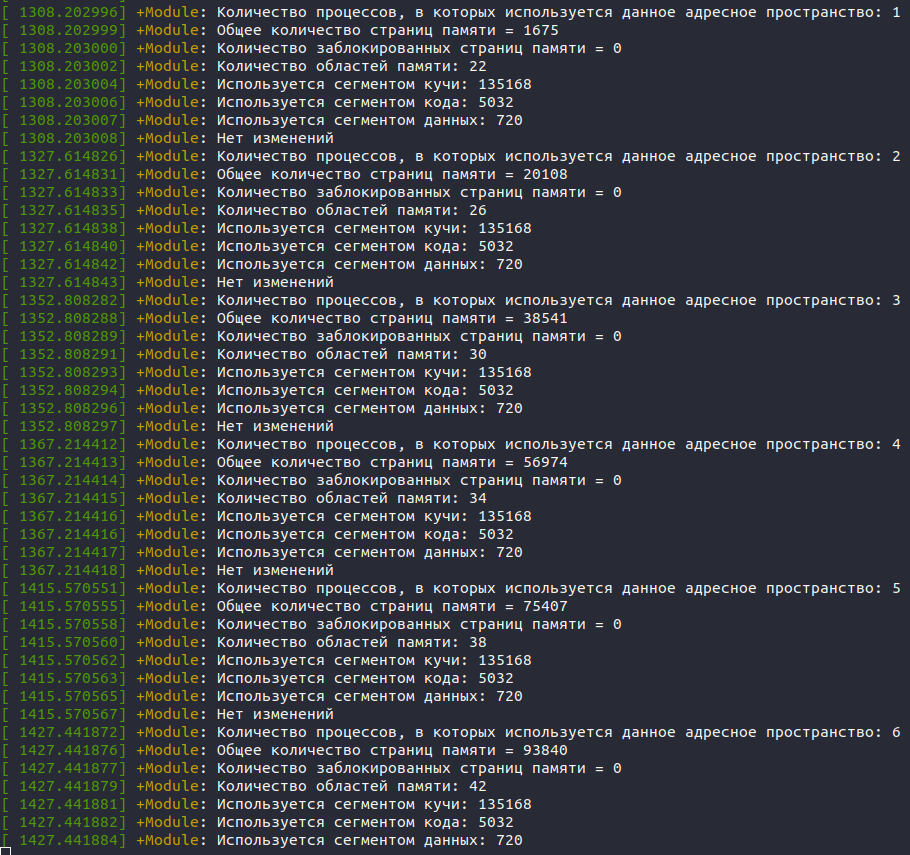
\includegraphics[width=0.95\textwidth]{img/analysis_pthread_count.png}
		\caption{Демонстрация увелечения количества страниц от количества потоков}
		\label{fig:analysis_pthread_count}}
\end{figure}

\newpage

% TODO: Указать размер  выделяемой памяти

\section{Анализ увелечения количества страниц программы, описанной выше}

На рис. \ref{fig:analysis_program} демонстрируется увеличение количества страниц 
при анализе описанной выше программы (при одном потоке).

Видно, что программе выделяется 33 страницы. 
Так же видно, что увеличивается размер кучи. 
Он увеличивается на 135168, что равно 33 * 4 * 1024, т.е. все 33 страницы выделяются под кучу.

\begin{figure}[ht!]
	\centering{
		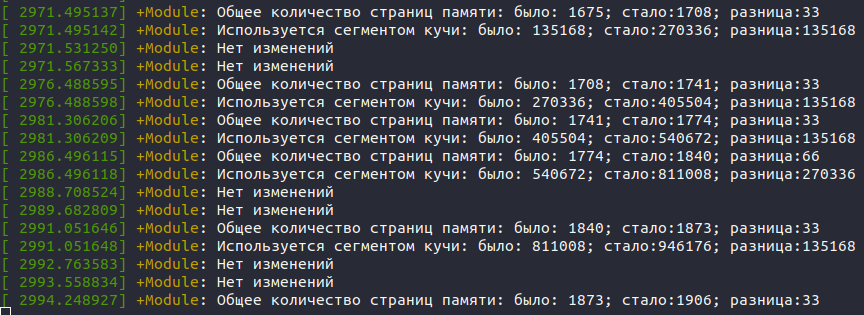
\includegraphics[width=1\textwidth]{img/analysis_program.png}
		\caption{Демонстрация увеличение количества страниц при анализе описанной выше программы}
		\label{fig:analysis_program}}
\end{figure}

\newpage

\section{Анализ увелечения количества страниц программы, описанной выше при увеличении количества потоков}

На рис. \ref{fig:analysis_program2} демонстрируется увеличение количества страниц 
при анализе описанной выше программы при увеличении количества потоков от 1 до 4.

Видно, что независимо, от изначального количества потоков программе выделяется 33 страницы. 

\begin{figure}[ht!]
	\centering{
		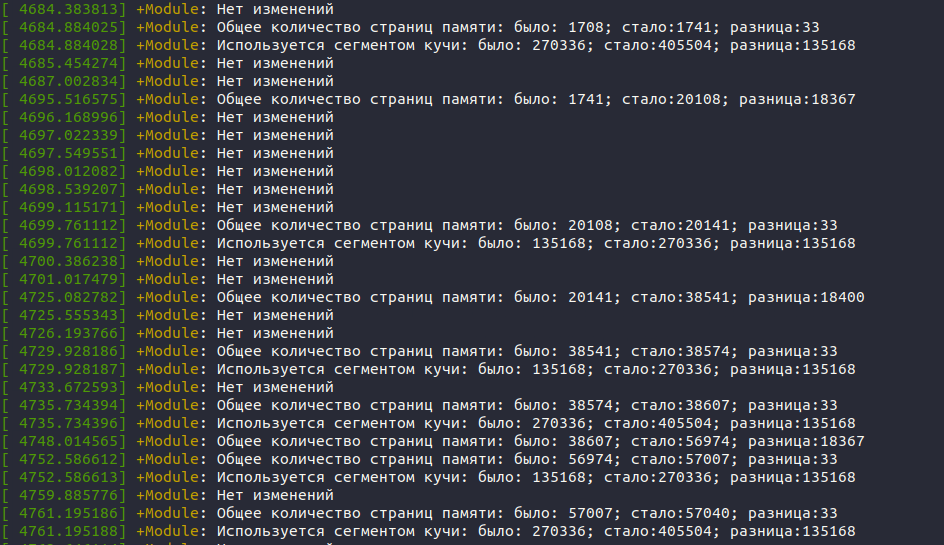
\includegraphics[width=1\textwidth]{img/analysis_program2.png}
		\caption{Демонстрация увеличение количества страниц при анализе описанной выше программы при увеличение кол-ва потоков}
		\label{fig:analysis_program2}}
\end{figure}

\section{Анализ вспомогательной программы}

На рис. \ref{fig:prog_2_1} запрашивается последовательно некоторое количество памяти,
размер которой в сумме дает 33 * 4 * 1024 байта, что равно 33 страницам.
Когда запрашиваемое количество памяти превышает 33 страницы, то общее 
количество страниц увеличивается на 33 
страницы см. рисунок \ref{fig:prog_2_2}. 

\begin{figure}[ht!]
	\centering{
		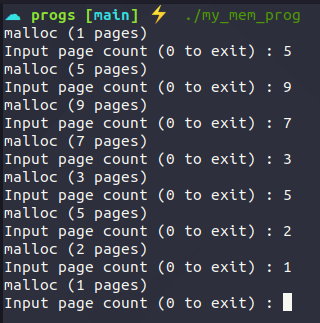
\includegraphics[width=0.6\textwidth]{img/prog_2/1.png}
		\caption{Последовательный запрос малого количества страниц}
		\label{fig:prog_2_1}}
\end{figure}


\begin{figure}[ht!]
	\centering{
		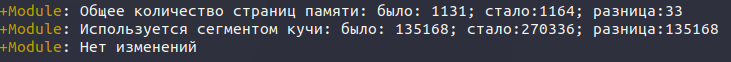
\includegraphics[width=1\textwidth]{img/prog_2/2.png}
		\caption{Результат при последовательном запросе малого количества страниц}
		\label{fig:prog_2_2}}
\end{figure}

\newpage

% Далее проанализируем запрос памяти, размер которой равен 30 страницам рис. \ref{fig:prog_2_3}.
% При первом запросе 30 страниц не выделяется новое кол-во страниц, т.к. оно не превышает 33.
% При следующем запросе 30 страниц выделяется 60 страниц. 
% Результат продемонстрирован на рис. \ref{fig:prog_2_4}.

% \begin{figure}[ht!]
% 	\centering{
% 		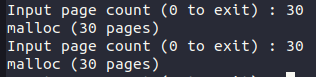
\includegraphics[width=0.6\textwidth]{img/prog_2/3.png}
% 		\caption{Последовательный запрос 30 страниц}
% 		\label{fig:prog_2_3}}
% \end{figure}


% \begin{figure}[ht!]
% 	\centering{
% 		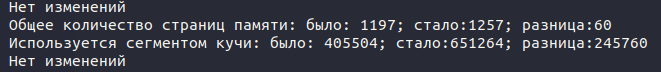
\includegraphics[width=1\textwidth]{img/prog_2/4.png}
% 		\caption{Результат при последовательном запросе 30 страниц}
% 		\label{fig:prog_2_4}}
% \end{figure}

% \newpage

На рисунках \ref{fig:prog_2_5} - \ref{fig:prog_2_10} показано, что при запросе памяти, 
размер которой более 33 * 4 * 1024 байта, что равно 33 страницам, общее количество страниц 
увеличивается на количество запрашиваемых страниц + 1.

\begin{figure}[ht!]
	\centering{
		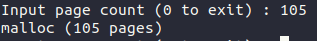
\includegraphics[width=0.6\textwidth]{img/prog_2/6.png}
		\caption{Запрос 105 страниц}
		\label{fig:prog_2_5}}
\end{figure}


\begin{figure}[ht!]
	\centering{
		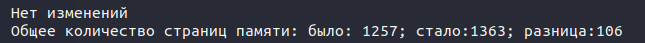
\includegraphics[width=1\textwidth]{img/prog_2/7.png}
		\caption{Результат при запросе 105 страниц}
		\label{fig:prog_2_6}}
\end{figure}

\begin{figure}[ht!]
	\centering{
		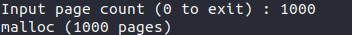
\includegraphics[width=0.6\textwidth]{img/prog_2/8.png}
		\caption{Запрос 1000 страниц}
		\label{fig:prog_2_7}}
\end{figure}


\begin{figure}[ht!]
	\centering{
		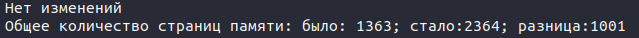
\includegraphics[width=1\textwidth]{img/prog_2/9.png}
		\caption{Результат при запросе 1000 страниц}
		\label{fig:prog_2_8}}
\end{figure}

\begin{figure}[ht!]
	\centering{
		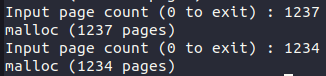
\includegraphics[width=0.6\textwidth]{img/prog_2/10.png}
		\caption{Запрос 1237 и 1234  страниц}
		\label{fig:prog_2_9}}
\end{figure}


\begin{figure}[ht!]
	\centering{
		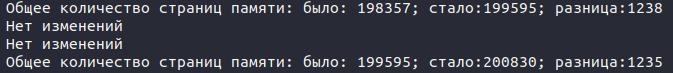
\includegraphics[width=1\textwidth]{img/prog_2/11.png}
		\caption{Результат при запросе 1237 и 1234 страниц}
		\label{fig:prog_2_10}}
\end{figure}

\newpage

\section{Вывод}

В данном разделе был приведен анализ общего количества выделенных страниц в 
зависимости от запрашиваемого количества памяти. Была проанализирована описанная выше программа.